\documentclass[11pt, oneside]{amsart}   	% use "amsart" instead of "article" for AMSLaTeX format
\usepackage[margin=1in]{geometry}
\usepackage[]{algorithm2e}
\geometry{letterpaper}
\usepackage{graphicx}
\usepackage{parskip}
\usepackage{amsthm, amsmath, amssymb}

\usepackage{listings}
\usepackage{xcolor}

\usepackage[all]{nowidow}

\definecolor{codegreen}{rgb}{0,0.6,0}
\definecolor{codegray}{rgb}{0.5,0.5,0.5}
\definecolor{codepurple}{rgb}{0.58,0,0.82}
\definecolor{backcolour}{rgb}{0.95,0.95,0.92}

\lstdefinestyle{mystyle}{
    backgroundcolor=\color{white},   
    commentstyle=\color{codegreen},
    keywordstyle=\color{blue},
    numberstyle=\tiny\color{codegray},
    stringstyle=\color{codepurple},
    basicstyle=\ttfamily\footnotesize,
    breakatwhitespace=false,         
    breaklines=true,                 
    captionpos=b,                    
    keepspaces=true,                 
    numbers=right,                    
    numbersep=5pt,                  
    showspaces=false,                
    showstringspaces=false,
    showtabs=false,                  
    tabsize=2
}

\lstset{style=mystyle}

\usepackage[final, colorlinks = true, 
            linkcolor = blue, 
            citecolor = black,
            urlcolor = blue]{hyperref} % For hyperlinks in the PDF

\graphicspath{ {images/} }

\usepackage{datetime2} % Uses YEAR-MONTH-DAY format for dates


%SetFonts
\usepackage{fancyhdr} % Headers and footers

\begin{document}

\title{Homework 4} % Article title
\fancyhead[C]{}
\begin{minipage}{0.295\textwidth} % Left side of title section
\raggedright
CS383: Databases\\ % Your lecture or course
\footnotesize % Authors text size
%\hfill\\ % Uncomment if right minipage has more lines
Isabelle Sanford % Your name
\medskip\hrule
\end{minipage}
\begin{minipage}{0.4\textwidth} % Center of title section
\centering 
\large % Title text size
Homework 4\\ % Assignment title and number
\normalsize % Subtitle text size
Sanderson Elimination Data Stuff \\ % Assignment subtitle
\end{minipage}
\begin{minipage}{0.295\textwidth} % Right side of title section
\raggedleft
\today \\
\footnotesize % Email text size
%\hfill\\ % Uncomment if left minipage has more lines
isanford@brynmawr.edu% Your email
\medskip\hrule
\end{minipage}

\section{Database Structure}

\subsection{Original data}

First, a brief review of the two original data sets I'm pulling from. For details on what particular columns mean, refer to the webpage from homework 3. (The columns listed aren't precisely the same as the ones below, but there's no massive structural change or anything.)


\subsubsection{Games}
Each row on the Games table represents a single game and collected data about it. A few of these columns aren't actually filled out right now (and others are very incomplete), but I'd rather include them in the structure now than try to add them later. Those are marked with a \textbf{*}. There are also several columns in the original sheet which were just aggregated from the Data sheet; I've left out most of those but there were a few that were useful to keep around for Mongo. 

\begin{itemize}
    \item \textit{Identifiers}: format, number, game string, anon number
    \item \textit{Forum thread}: title, link*, \# posts, start date*, end date*
    \item \textit{Summary stats}: \# players, \# eliminators, \# survivors
    \item \textit{Game structure}: fundamentals, complexity, role madness*
    \item \textit{Game results}: winner, mechanics balance*, distribution balance*
    \item \textit{Other}: GM(s), IM, \# cycles, setting
\end{itemize}

The notable changes since HW3 is that `Broken' was split into two separate balance columns, and we've added several columns about various aspects of the game's fundamental structure. (`Role madness' means everyone in the game gets a role/ability.)

\subsubsection{Player Data}
The Player Data table is the majority of the raw data. It contains one row for every player that interacted with any game: that is, a particular game would have a bunch of rows containing the data for each player in that game, and then additional rows indicating who ran and supervised that game. This table is currently about 5000 rows. It's mostly filled out, with the exception of the `role' columns which are only about a quarter full. 

\begin{itemize}
    \item \textit{Identifiers}: ID, player name, game format / number / string 
    \item \textit{Category}: alignment (if playing), or GM, Main GM?, Mod (for non-players)
    \item \textit{Results}: faction outcome, death/survival outcome, went\_inactive, role*, secondary role*
    \item \textit{Hits}: first hit (i.e. first cycle attacked), last hit, total \# of hits
\end{itemize}

Changes from HW3 are the roles columns and a boolean `Main GM?' column indicating whether someone was the primary person running the game or just helping out. 


\subsection{Mongo}

Let's start with Mongo, since the structure of that database is much more similar to the original data. The database contains two collections: \texttt{players} and \texttt{games}, since those are the two major entry points for asking questions about the data. They do contain overlapping information (because it's mongo), though arguably not as much as they should. I'll admit that I put much less effort into these than the SQL data, partly because I didn't have to worry as much about messy data, but mainly because I like SQL better and plan to use that SQL database past the end of this course and throw this one out. Given more time and interest, these collections should be somewhat more robust, each containing almost all of the total information. 


\subsubsection{games}
The \texttt{games} data is actually fairly close to what the original Games table contained, and looks approximately like this: 

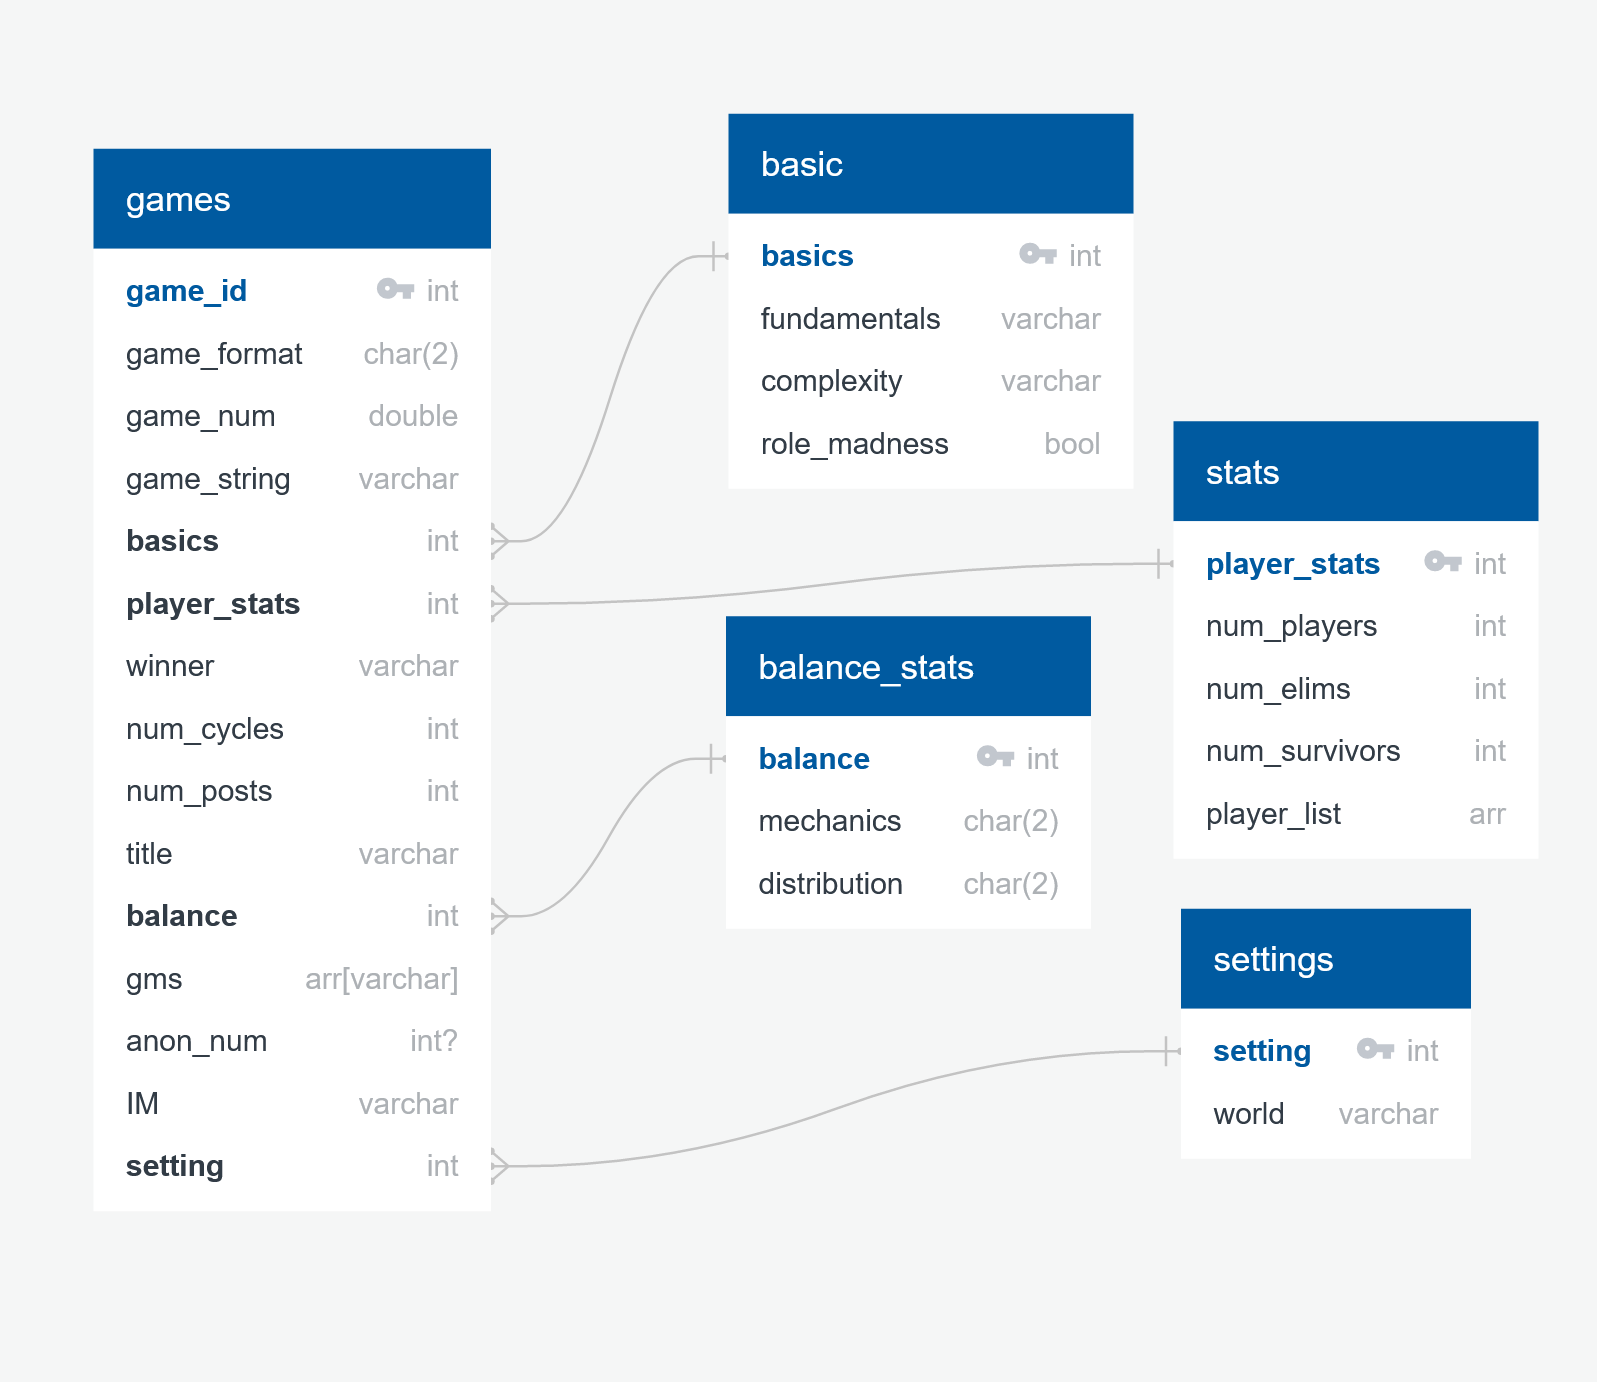
\includegraphics[scale=0.5]{../mongo/mongo_games_v0.png}

I've included an example below (real data, truncated for space), but essentially the Game data is split into sensible categories (similar to those listed on page 1), and there's a player list pulled from the original Player Data. That player list doesn't contain any stats about what happened to the player in that game (although it arguably should), but a name is enough to look up the relevant data from the \texttt{players} collection. I've also kept some of the summary stats (like the number of players) in Mongo, for easy access to especially common ones without having to cross-reference with \texttt{players}. There's an index on the ``format'' option, as filtering by format will be fairly common and there are only five formats available. 

\begin{verbatim}
{'format': 'MR',
'game_num': 38.1,
'game_string': 'MR38.1',
'basics': {
    'fundamentals': 'U', 
    'complexity': 'Basic', 
    'role_madness': False
    },
'player_stats': {
    'num_players': 18.0,
    'num_elims': 5.0,
    'num_survivors': 15.0,
    'player_list': [
        'Haelbarde',
        'Straw',
        ...
        ]
    },
'winner': 'E',
'num_cycles': nan,
'num_posts': nan,
'title': 'The Council of Elrond',
'balance': { 'mechanics': nan, 'distribution': nan },
'setting': { 'world': 'Lord of the Rings' }
'GMs': ['Elbereth', 'Elbereth'],
'IM': 'little wilson'
}
\end{verbatim}
Note that there are also currently a lot of places where a document contains something like \texttt{"mechanics": nan}, which should really just be left out of the document altogether.

\subsubsection{players}
The \texttt{players} collection, on the other hand, isn't structured very like the original Player Data (though it contains almost exactly the same information). Instead, it's a version of that data aggregated by player, like so:

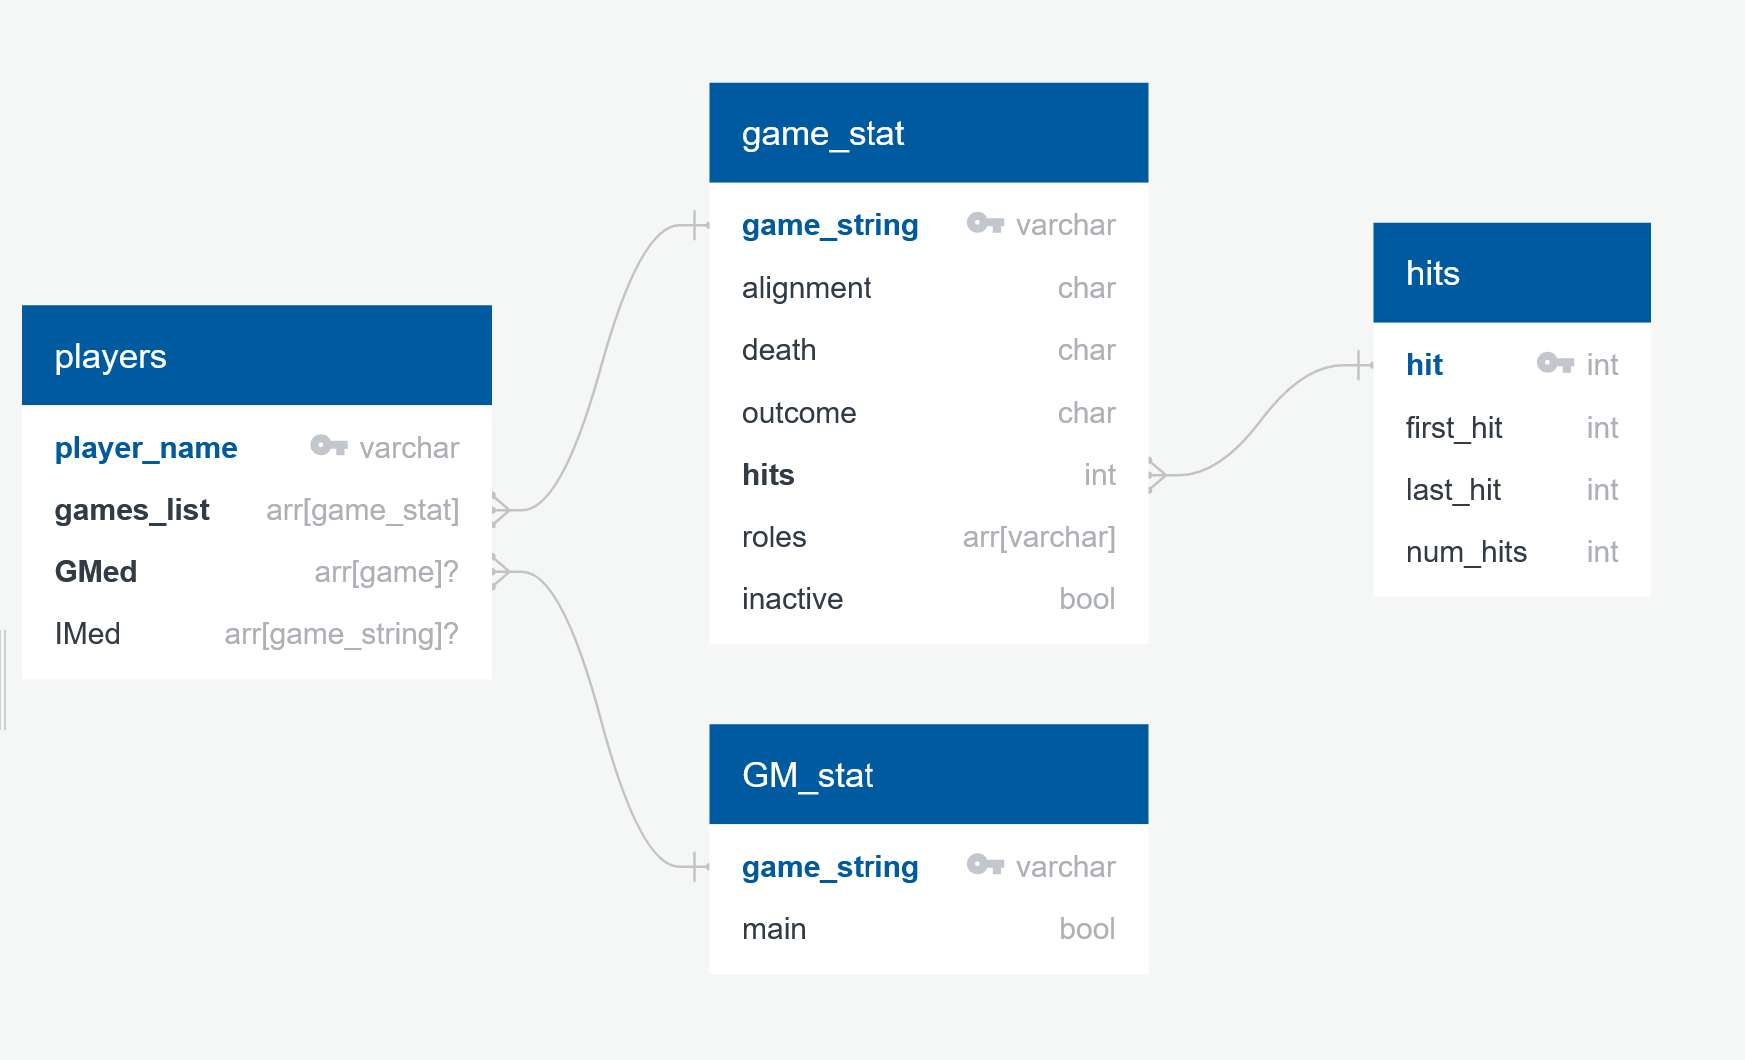
\includegraphics[scale=0.5]{../mongo/mongo_players_v0.png}

Again, I've included an example below, this time of my own document (again truncated for space). I've included an index on ``game\_string'' inside the list of games, since that string effectively serves as the primary key for the \texttt{games} collection whenever cross-referencing is needed. 

\begin{verbatim}
{'player_name': 'Elbereth',
'games': [
    {
        'game_string': 'LG15.2',
        'alignment': 'G',
        'death': 'S',
        'result': 'W',
        'hits': {
            'first': nan, 
            'last': nan, 
            'num': 0.0
        },
        'roles': ['Kill', nan],
        'inactive': False
    },
    ...
],
'GMed': [
    {'game_string': 'QF11', 'main': False},
    {'game_string': 'LG19', 'main': True},
    ...
],
'IMed': [
    {'game_string': 'MR42'},
    {'game_string': 'LG68'},
    {'game_string': 'LG70'},
    ...
]}
\end{verbatim}

Though it was true to an extent in the last collection, it's much more noticeable in this one that you need some outside knowledge to decipher what's going on, particularly for the alignment/death/result values. Those characters are based on key tables from the original spreadsheet, present in the SQL database but absent here - rather than having a separate table, the ideal case would be to just replace those single characters with more descriptive strings like ``Good'' / ``Survived'' / ``Won'' and so on. 

There are two more possible lists in a single player's document. The one labeled `IMed' is fine as is; it's a list only present in the dozen or so people that have been forum moderators over the years, since each game gets supervised by one of them. It's not a statistic that's especially meaningful. The `GMed' list, on the other hand, is something that could and probably should be a little more extensive. The original Player Data sheet only provides the two fields shown there without a bunch of aggregation, and `game\_string' could be used as a key to look up any of the games in the \texttt{games} collection, but it'd still maybe be convenient to have a little more summary information here for games that the player has run rather than having to deal with joins. 

\subsection{SQL}

For putting all this into SQL, I went much more heavy on splitting out things, making key tables, etc, so the final structure looks like this: 

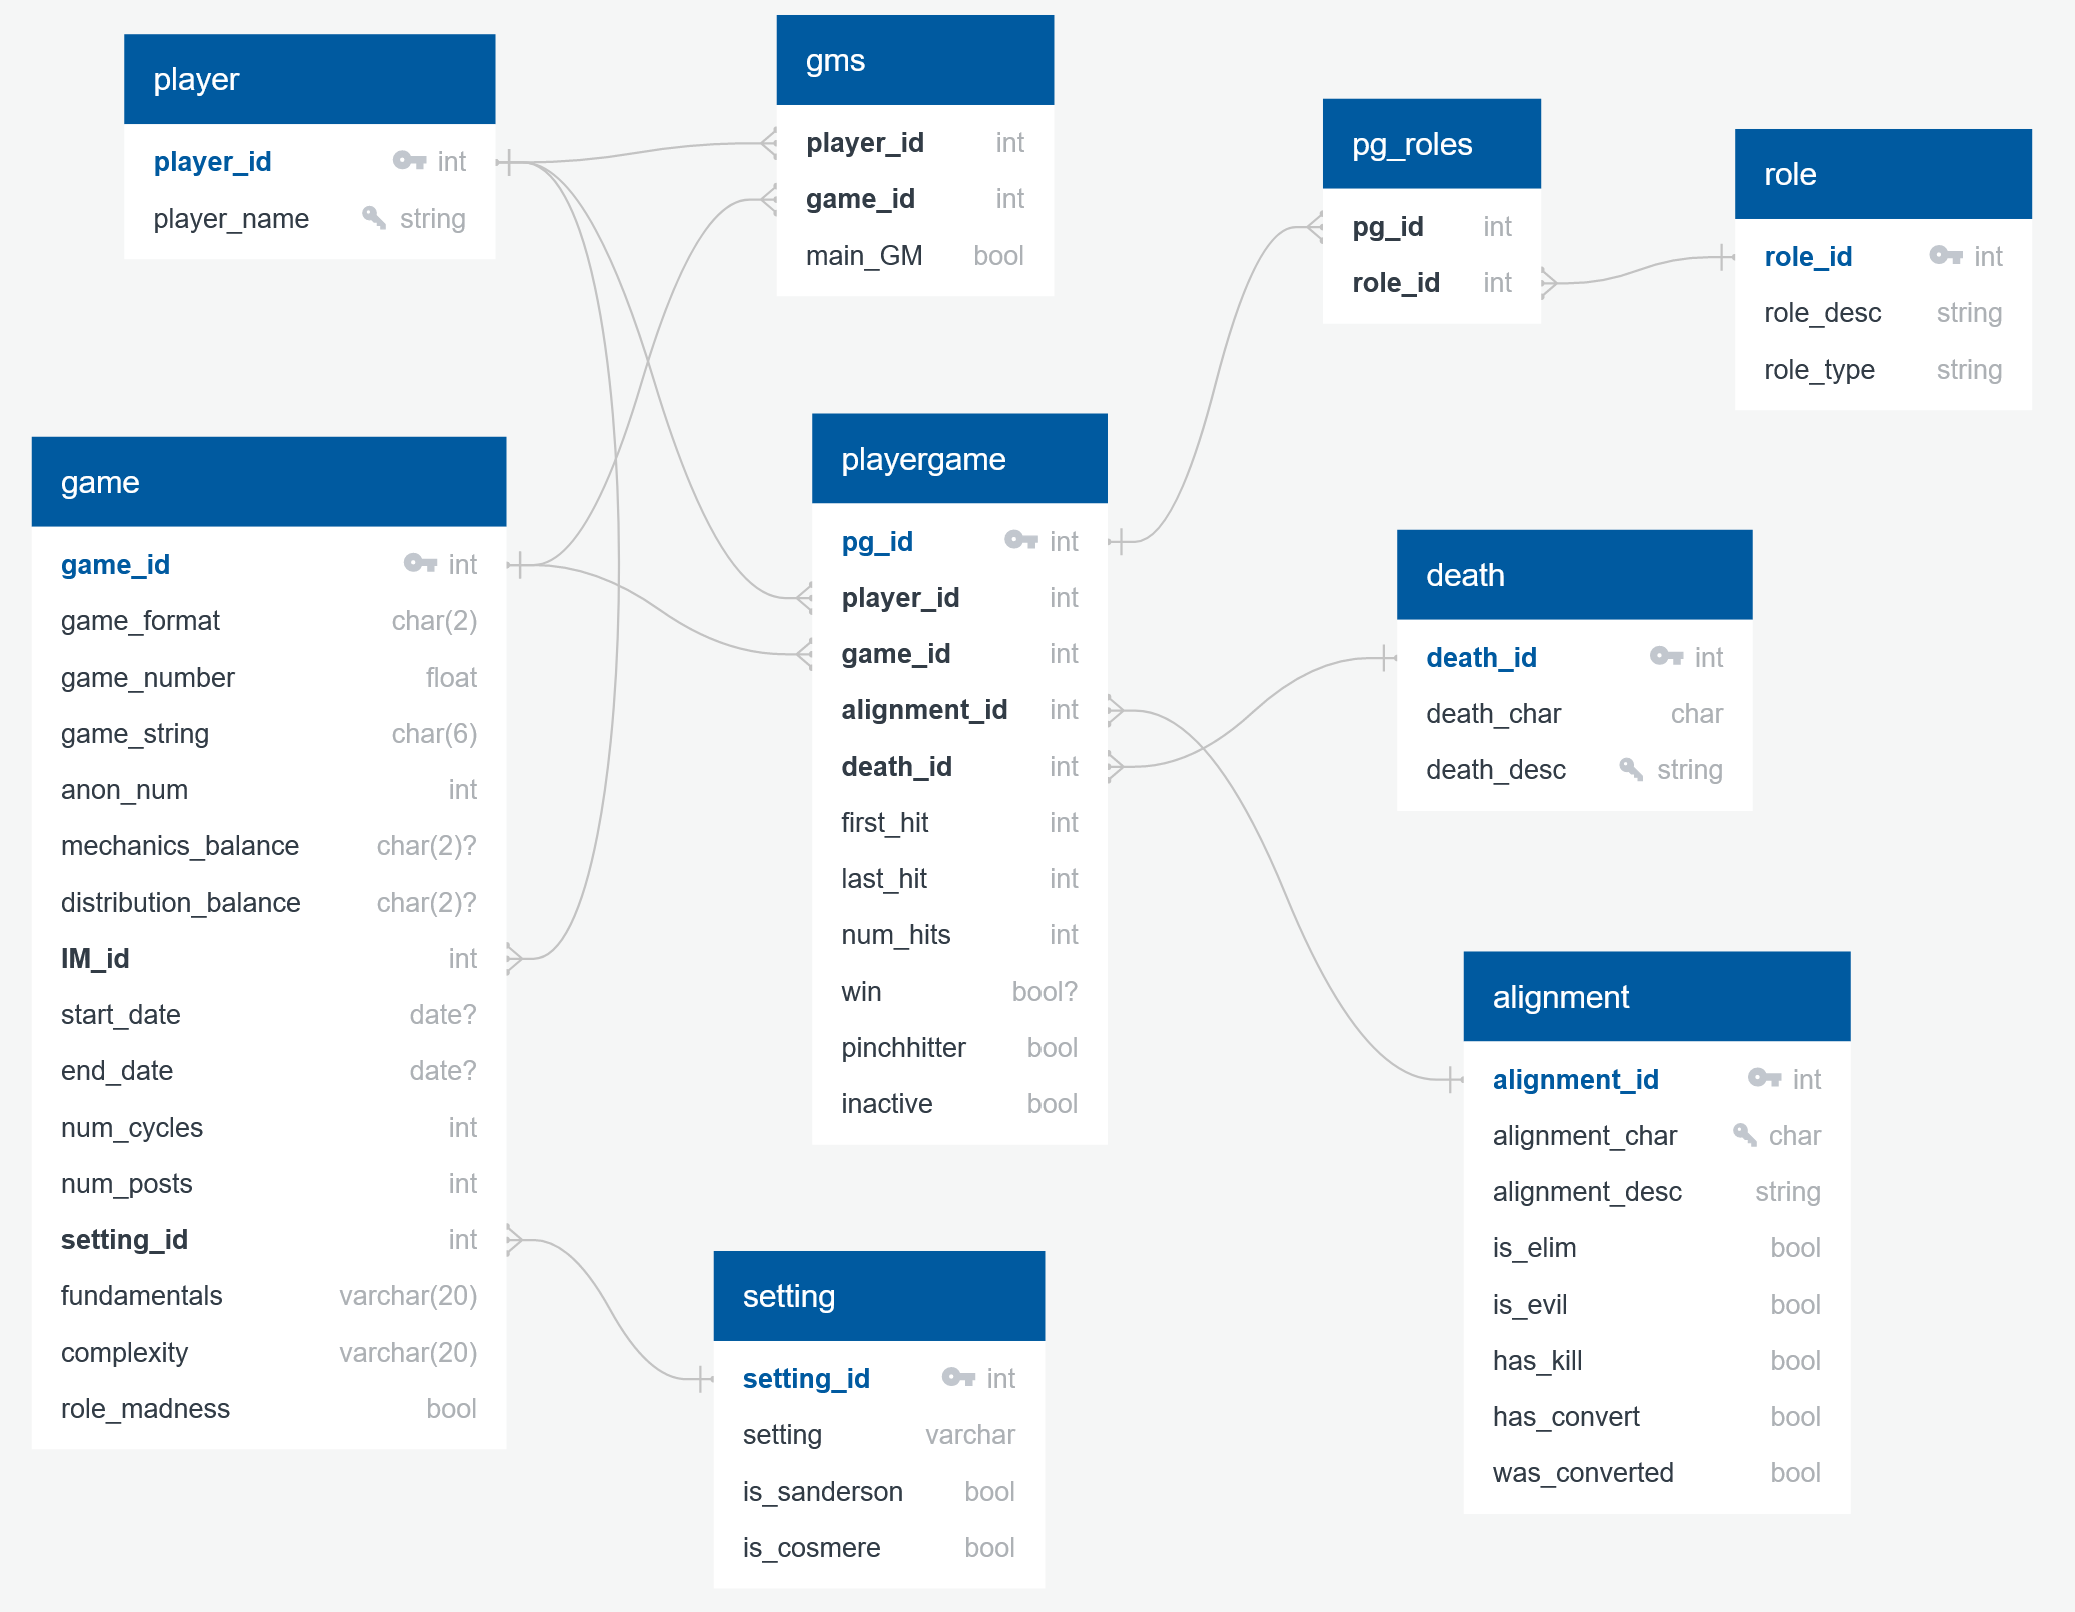
\includegraphics[scale=0.5]{../diagrams/se diagram v3.png}

Each player, game, alignment (i.e. team), death type, game setting, and role gets its own integer primary key in separated out key tables. That's most important for \texttt{player}, as players are both referenced all over the place and often change their name over time. (In the spreadsheet, we just have to do a find-and-replace and hope nothing goes wrong.) 

The \texttt{game} table looks somewhat like the original game data, as most of that table is in fact data that applies only to the game in question or that doesn't need any information attached. The only notable key table connection there is to \texttt{setting}, since it's helpful to hold a couple of booleans about each setting in addition to the setting itself for easy querying. (That said, I could also have made key tables for the two balance columns, the fundamentals column, and the complexity column. I didn't partly because those would be very tiny tables, but mostly because those columns are currently in flux in the spreadsheet and may not end up structured as they are right now.)

The \texttt{playergame} table contains very similar information to the original Player Data table, and is still a few thousand rows (not quite the full five thousand since GMs, IMs, etc have been moved to their own spots), but now nearly half the columns are integers that connect to varying key tables. Some of these aren't very interesting (the \texttt{death} table doesn't currently contain any information that wouldn't be as easily gathered by just putting the death description into \texttt{playergame}), but some of them (like \texttt{alignment}) have a bunch of extra data that makes certain queries much easier. For instance, there are seven different types of evil teams, each of which has their own id. Having an is\_evil boolean is much, much nicer than having to specify all seven options.

There's also an index in the \texttt{playergame} table on `player\_id', which is one major grouping of the table. (There could arguably be a useful one on `game\_id' too, which would be something like a btree rather than hashed.)

As I mentioned, the \texttt{gms} table has been separated out. It would be more intuitive to just have a GM attribute inside \texttt{game}, but the problem is that there can be (and often are) multiple GMs running a single game. So to avoid duplication, there's a small table with just a player and a game they ran in each row, plus a boolean indicating whether they were the ``main'' GM or not. 

The last branch I haven't described here is the \texttt{pg\_roles} table and its associated \texttt{role} key table. These are the most tentative tables, mainly because we only recently started collecting role data and less than a quarter of the data is filled in right now. But the idea is that a player sometimes has multiple roles in a single game, which means putting roles into \texttt{playergame} wouldn't work without duplication somewhere or using arrays. Instead, I gave \texttt{playergame} a primary key ID, and the idea is for \texttt{pg\_roles} to list roles which a certain player in a certain game had. Currently both the \texttt{roles} and the \texttt{pg\_roles} tables are empty, because cleaning those up enough to insert is lower priority than, say, my number theory homework. 

Since the data does now take a fair amount of joining to make it human-understandable, I'm planning on (but have not yet made) a materialized view that has some summary stats and the real names of things, replicating some of the parts of the original sheet. 


\section{Queries}

\subsection{Question:} What games have I (``Elbereth'') played? 
This uses the SQL index on players in playergame, so it can easily find which rows are me without necessarily having to search through every entry. It uses the index in Mongo on the list of game strings for each player, although the index is more intended for use when cross-referencing the games table. 

SQL answer: 
\begin{lstlisting}[language=SQL]
with my_games as (
    select game_id from playergame 
    where playergame.player_id IN (
        select player_id from player where player_name LIKE 'Elbereth'
    )
)
    
select game_string from game natural join my_games;
\end{lstlisting}
    
Mongo answer:
\begin{lstlisting}[language=java]
db.players.findOne(
  { player_name: "Elbereth" },
  { "games.game_string": 1, _id: 0 }
);
\end{lstlisting}

\subsection{Question:} How often do evil teams win? 
Note that for this question and the next, the answers in Mongo and SQL will be slightly different because Mongo is pulling from the ``winner'' column from the original Games sheet, which only allows one winner to be marked per game (when there can be multiple). The SQL is the more accurate (and that's partly why the SQL is more complex, though some of that is also definitely me being inelegant). 

SQL answer:
\begin{lstlisting}[language=SQL]
with e_games as (
    select win, count(distinct game_id) as elim_results
        from playergame as pg
        where alignment_id in (select alignment_id from alignment where is_elim)
        group by win
),

all_games as (select sum(elim_results) as num_e_games from e_games),

won_games as (select sum(elim_results) as won from e_games where win)

select (won / num_e_games) as elim_win_perc from all_games, won_games;
\end{lstlisting}
(The answer, according to SQL, is about 52\%.)

Mongo answer:
\begin{lstlisting}[language=java]
db.games.find({ winner: "E" }).count() / db.games.count();
\end{lstlisting}

\subsection{Question:} Do games where the evil team wins last longer/shorter than when they don't? (More broadly - does which team won correlate any with game length?)

SQL answer:
\begin{lstlisting}[language=SQL]
-- all factions that won for each game and how many people 
WITH by_game AS (
    select game_id, alignment_id
    from playergame
    where win
    group by game_id, alignment_id
),

-- above with cycle length for each game
with_nums AS (
    SELECT * 
    FROM by_game 
        NATURAL JOIN (select game_id, num_cycles from game) AS cycle_nums
), 

-- grouped by alignment
by_alignment AS (
    SELECT alignment_id, avg(num_cycles) as avg_cycle, count(num_cycles) as num_games
    FROM with_nums 
    GROUP BY alignment_id
)

-- adding alignment description
SELECT alignment_desc, avg_cycle, num_games, is_evil 
    FROM by_alignment NATURAL JOIN alignment;
\end{lstlisting}


Mongo answer:
\begin{lstlisting}[language=java]
db.games.aggregate([
    {
        $group: {
        _id: "$winner",
        avgCycles: {
            $avg: "$num_cycles",
        },
        },
    },
    ]);
\end{lstlisting}



\end{document}


